\subsection{Instancias propuestas}

En la siguiente sección analizaremos tres instancias distintas del sistema.

Estas consisten en:
\begin{itemize}
    \item{Un horno muy frío (temperatura interior: 1500, temperatura exterior: 30)}
    \item{Un horno muy caliente (temperatura interior: 1500, temperatura exterior: 480)}
    \item{Un horno averiado, que para la mitad superior esté muy caliente y para la mitad inferior muy frío}
\end{itemize}

Para todos los casos, la isoterma buscada es de 500 grados.

La utilidad de estos tres casos es para mostrar que el tiempo de resolución del sistema no depende de los valores del mismo, sino de cómo se discretiza el horno. El tercer caso nos resulta interesante, además, para ver cómo varía la isoterma al tener tan marcada la diferencia de temperatura. 

\subsection{Análisis de isoterma}

En la figura \ref{exp1-hfhc} podemos ver un gráfico de los hornos y su respectiva isoterma. Previamente explicamos cómo se calcula esta isoterma y en los gráficos podemos ver esto reflejado. Para el horno caliente, podemos observar que la isoterma está cerca de las paredes. Esto es porque las paredes externas tienen una temperatura de $480$. Para el horno chico, vemos que la isoterma se encuentra más bien lejos de las paredes externas, pues estas se encuentran frías.  

\begin{figure}[!htb]
    \caption{Izquierda: Horno Caliente, Derecha: Horno Frío}
    \label{exp1-hfhc}
\centering
\minipage{0.5\textwidth}

  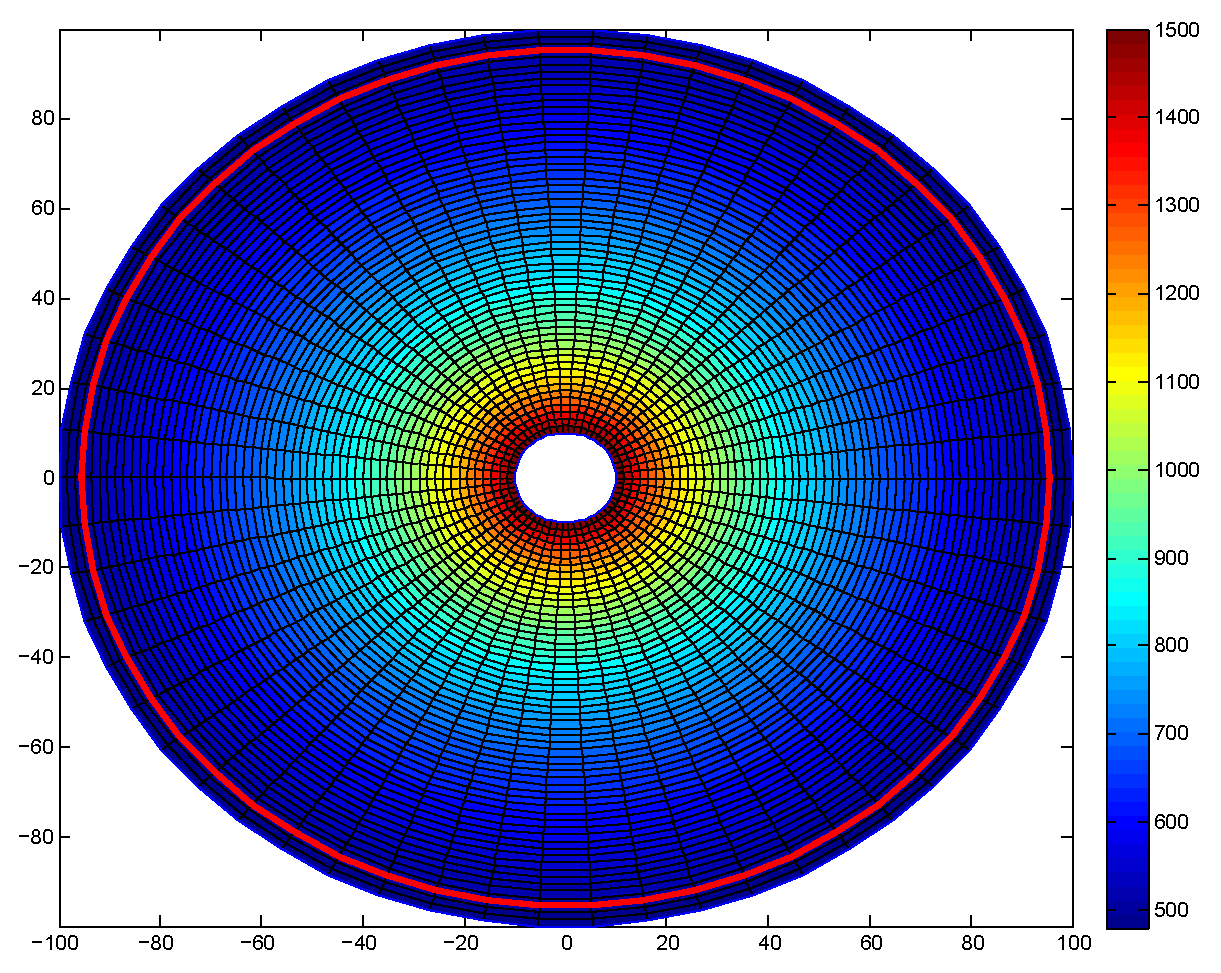
\includegraphics[width=1\textwidth]{figures/calor-isoterma-mn19.pdf}

\endminipage\hfill
\minipage{0.5\textwidth}

  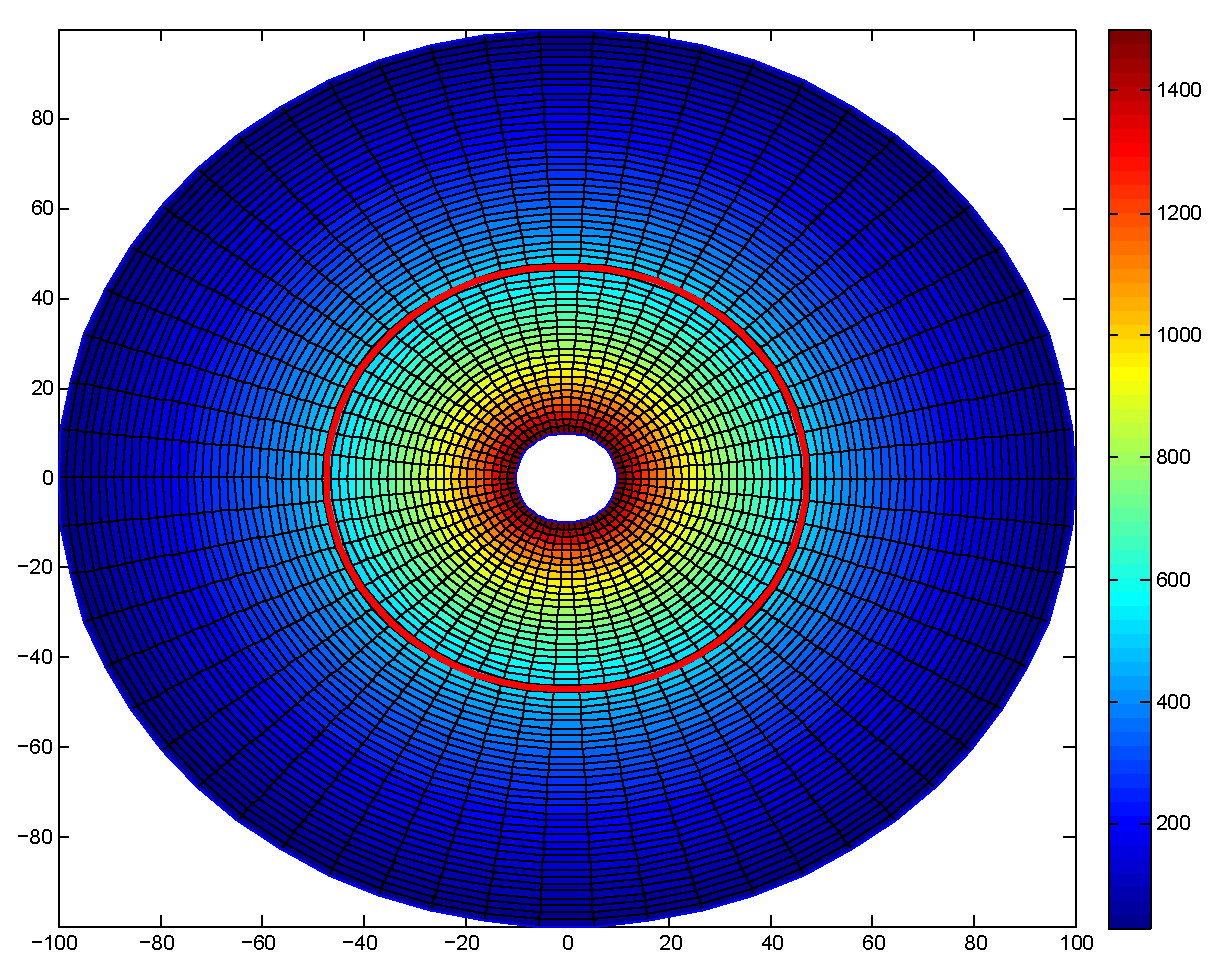
\includegraphics[width=1\textwidth]{figures/frio-isoterma-mn19.pdf}

\endminipage\hfill
\end{figure}

\clearpage
\begin{figure}[!htb]
    \caption{Horno con parte inferior caliente y parte superior fría}
    \label{exp1-hfc}
\centering
  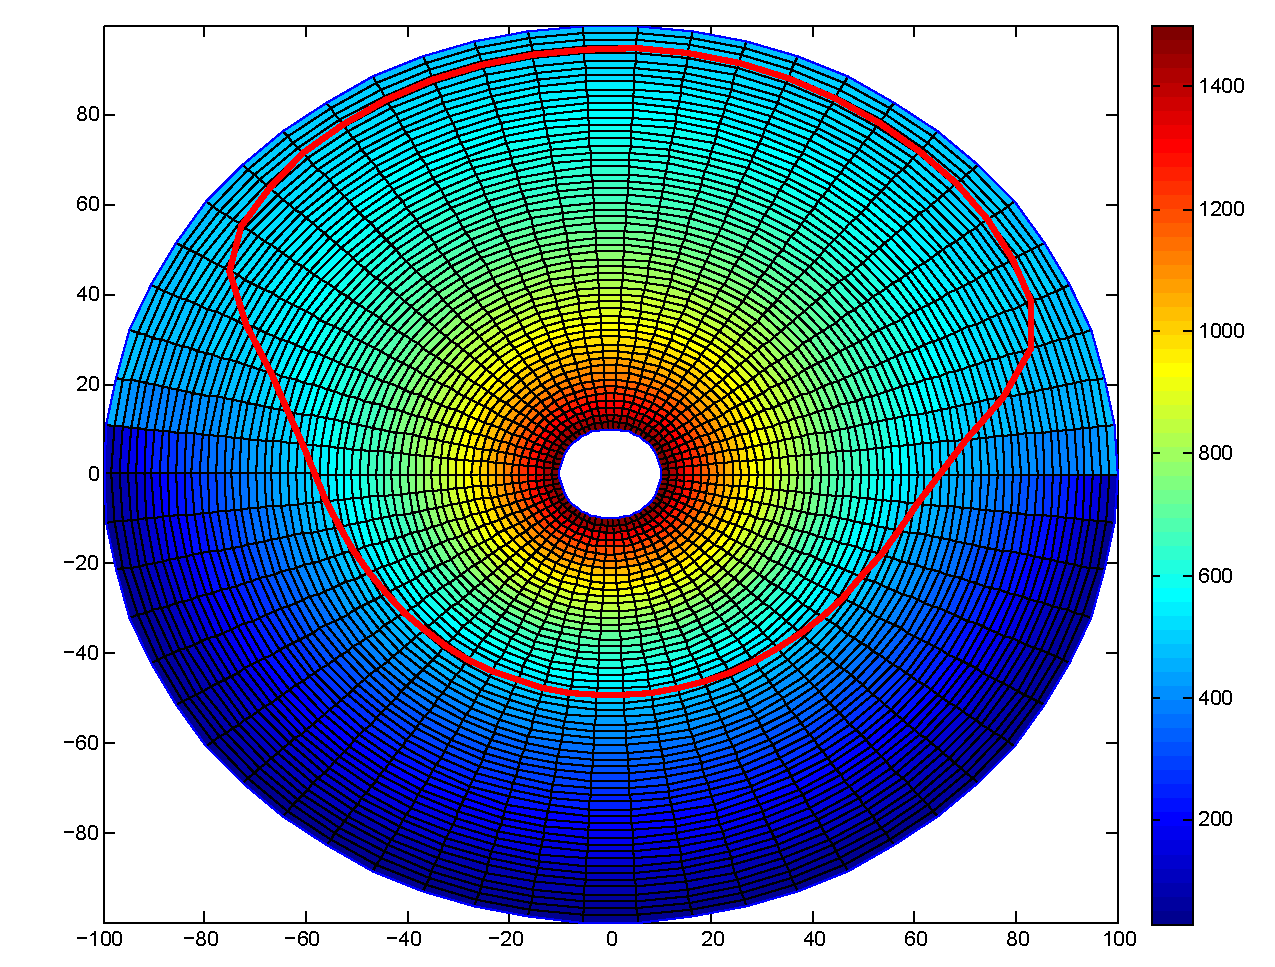
\includegraphics[width=0.75\textwidth]{figures/friocalor-isoterma-mn19.pdf}
\end{figure}

Un caso más interesante es el de la figura \ref{exp1-hfc}, donde la temperatura no es igual en todos los ángulos medidos. En el gráfico del horno se puede ver cómo la parte superior está más caliente que la inferior, y cómo la isoterma se va adaptando, moviendose entre casillas de colores muy similares, en la escala de la derecha podemos ver que el color por donde pasa la isoterma está muy cerca del color de la temperatura correspondiente a $500$.

~

\clearpage
\subsection{Análisis de performance}
\subsubsection{Medición de ciclos de procesador}

Para realizar las mediciones y comparaciones, en vez de medir los tiempos de inicio y final, utilizamos un método sugerido por Intel [Intel-1]\footnote{El paper sugiere más técnicas además de las que utilizamos nosotros para mejorar el monitoreo de performance: Correr el programa en un módulo de kernel sin desalojo y medir cuánto overhead tiene la llamada a rdtsc. Eso es útil cuando se desea una granularidad extrema de menos de 1000 cicos de procesador, nosotros no necesitamos tanta granularidad}, contando los ciclos de procesador utilizando la instrucción de procesador \textbf{RDTSC}. Tuvimos en cuenta las siguientes cosas:

\begin{itemize}
    \item Todas las mediciones fueron realizadas 10 veces, y luego se promediaron los valores
    \item Se corrieron los experimentos en un sistema multicore
    \item En vez de realizar una llamada a función, utilizamos una macro que usa inline-assembly para diminuir el overhead de realizar la medición en sí.
    \item Creamos una barrera de ejecución con la instrucción lfence para evitar que el procesador ejecutara instrucciones fuera de orden (es decir, para evitar que el procesador ejecutara rdtsc antes de haber terminado de ejecutar el programa). 
\end{itemize}

Consideramos que todos esos detalles nos brindan el nivel de precisión necesario para las mediciones del problema. 

En un sistema multiproceso como Linux es posible que no todos los ciclos de procesador sean destinados a nuestro proceso, tratamos de mitigar eso realizando los experimentos varias veces y luego promediando los ciclos insumidos, también ayuda el hecho de ejecutar el programa en un sistema multicore.

Decidimos utilizar una macro inline assembly y rdtsc ya que hay un overhead significante en llamar a funciones, y obtener el tiempo. Es posible que al obtener el tiempo actual se realize una \textbf{syscall} y esto desaloje nuestro proceso\footnote{A menos que el kernel implemente vDSO para la función de obtener el tiempo.}. Es cierto que para instancias grandes del problema, una diferencia de medio segundo es casi despreciable, pero consideramos que realizar las mediciones de esta forma disminuyen el error sin mucho esfuerzo.

Finalmente, la forma en la que utilizamos todo esto es: El programa cuenta los ciclos de reloj antes y despues de resolver el sistema (llamando a la macro que se puede encontrar en el archivo \textbf{tiempo.h}), los ciclos insumidos es el valor absoluto de la diferencia entre ciclos iniciales y finales. \footnote{notar que dado que usamos precisión de 64 bits, sólo es posible que haya overflow si la computadora estuvo prendida por más de 500 años}. 

\subsubsection{Benchmarks}


Realizamos una serie de pruebas para analizar la performance de la resolución del sistema. Hicimos las pruebas en las tres instancias descriptas previamente. Realizamos los tests variando la cantidad de puntos de discretizaci\'on que utilizamos, variando el $n$ (cantidad de \'angulos o sensores), el $m$ (cantidad de radios) y $n$ y $m$ al mismo tiempo. Medimos los resultados contando los ciclos de procesador insumidos. Por cada test corrimos $10$ repeticiones del mismo y luego promediamos los resultados, a modo de amortizar los ciclos de más por ser desalojados del scheduler. 

~

Esperamos que cada uno de los distintos escenarios insuman cantidades muy cercanas de ciclos en su resolución, ya que los valores de los datos deber\'ian ser irrelevantes para el tiempo de procesamiento. Adem\'as, el tiempo de procesamiento deber\'ia seguir un comportamiento cúbico en función de la entrada, ya que es esa es la complejidad del algoritmo utilizando eliminaci\'on Gausseana.

\begin{SCfigure}[1][ht!]
\sidecaptionvpos{figure}{t}
  \caption{ Se pueden observar los resultados de las primeras tres pruebas. Variamos $n$ (cantidad de angulos o sensores) en los tres escenarios que presentamos anteriormente utilizando eliminación Gausseana para resolverlos. Como se puede visualizar, el insumo de ciclos es cúbico en función de la cantidad de ángulos y la resolución de los tres escenarios insumió una cantidad muy cercana de ciclos, que es lo que estabamos esperando. \newline \newline}
  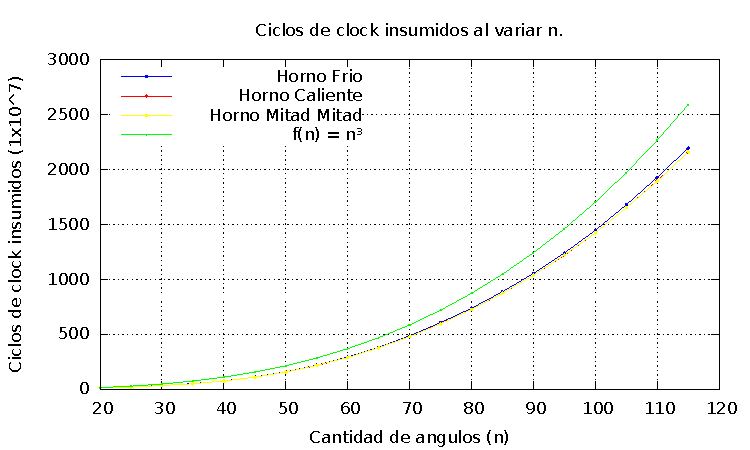
\includegraphics[width=0.6\textwidth]{../src/experimentacion/PDFs/sensores.pdf}
\end{SCfigure}

\begin{SCfigure}[1][ht!]
\sidecaptionvpos{figure}{t}
  \caption{ Al igual que la figura anterior, se puede observar exactamente el mismo comportamiento cuando solamente variamos $m$: un insumo de ciclos cúbico e insumos cercanos para los tres escenarios. \newline \newline \newline \newline \newline \newline \newline \newline}
  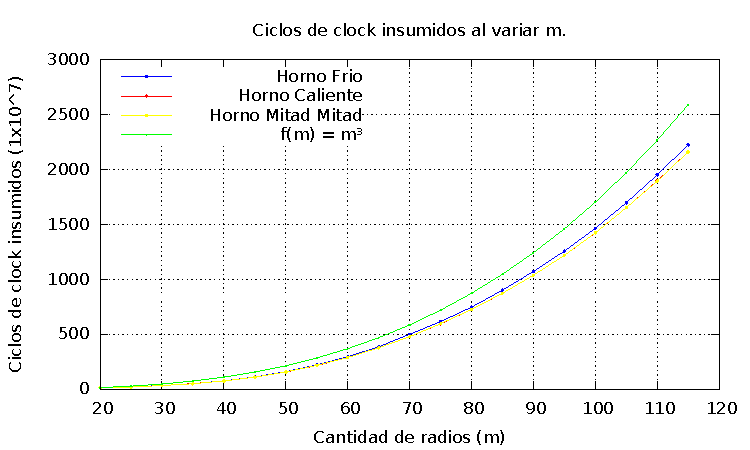
\includegraphics[width=0.6\textwidth]{../src/experimentacion/PDFs/radios.pdf}
\end{SCfigure}

\begin{SCfigure}[1][ht!]
\sidecaptionvpos{figure}{t}
  \caption{ Esta figura, si bien sigue la misma tendencia que las anteriores, es un poco distinta. Debido a la variación de ambos parametros la curva es mucho más cócava que en las experimentaciones anteriores. Sin embargo, los tres escenarios siguen insumiendo una cantidad similar de ciclos en cada instancia, que es lo que esperabamos ver.\newline \newline \newline \newline}
  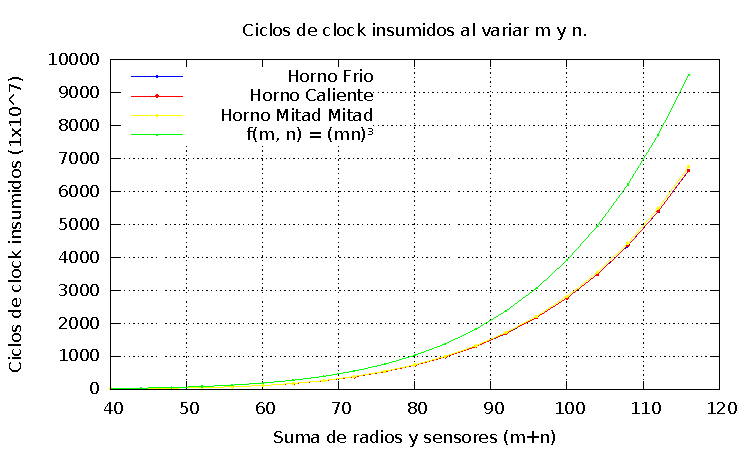
\includegraphics[width=0.6\textwidth]{../src/experimentacion/PDFs/ambos.pdf}
\end{SCfigure}

\newpage
\subsection{Factorización LU vs Eliminación Gaussiana}

En esta sección compararemos la performance de los dos métodos de resolución utilizados. Dado que LU factoriza una sola vez la matriz, resolver el mismo sistema cambiando solo las mediciones implica un menor costo que resolver todo el sistema nuevamente (cosa que sucede con el método de eliminación Gaussiana). Basándonos en este razonamiento, esperamos conseguir una mejora de performance por parte del método LU cuando hay que resolver varias instancias del mismo sistema.


Proponemos dos experimentos, el primero consiste calcular la isoterma para muchas instancias del mismo horno, pero variando la temperatura de los sensores, simulando un efecto de 'paso del tiempo', en donde las paredes externas del horno comienzan a calentarse desde un estado inicial con temperatura $0$. La evolución del estado del horno se puede apreciar en la figura \ref{exp2-hornos}. En la figura \ref{compbench-glu} mostramos la comparativa de ciclos insumidos por LU y Gauss, confirmando que conviene realizar LU cuando queremos analizar más de una instancia. Sin embargo, la cantidad de ciclos insumidos para la primer iteración es similar: el método LU debe factorizar la matriz y eso lleva casi lo mismo que el método de eliminiación gaussiana. 


El segundo experimento trata de mostrar cómo varían la performance en función del tamaño del sistema y de las iteraciones. Simulamos varios sistemas como el anterior (un horno calentándose), pero en cada sistema aumentamos la cantidad de radios de la discretización y la cantidad de instancias. Con esto esperamos poder mostrar que luego de resolver la primer instancia, el proceso de resolución de las instancias siguientes es mucho más rápido con LU que con Gauss. Esto se puede ver en la figura \ref{compbench-extra}.

~

\begin{figure}[!htb]
    \caption{Evolución del horno en función del tiempo. Se ve cómo la isoterma de $500$ grados se acerca hacia el borde del horno, hasta que lo supera.}
    \label{exp2-hornos}
\centering
\minipage{0.5\textwidth}

  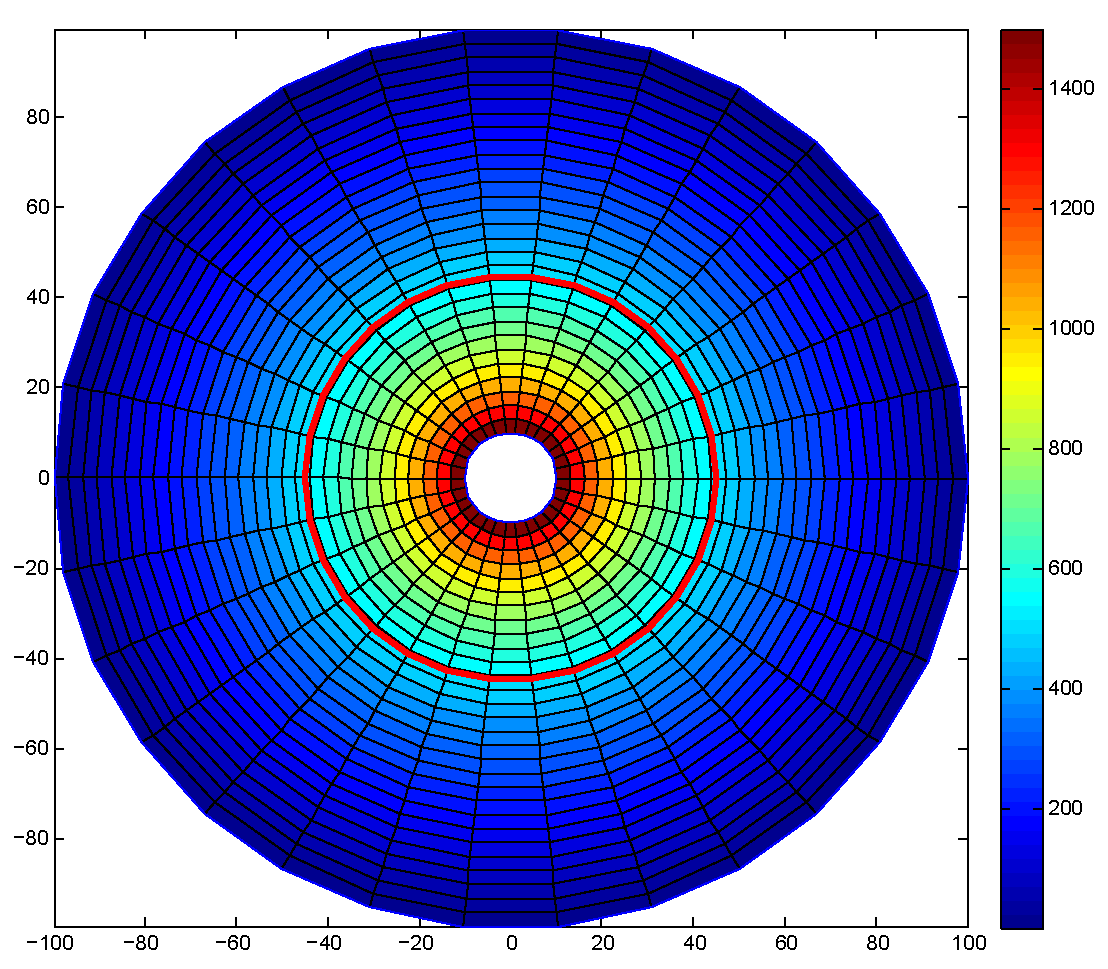
\includegraphics[width=1\textwidth]{figures/exp2-1.pdf}

\endminipage\hfill
\minipage{0.5\textwidth}

  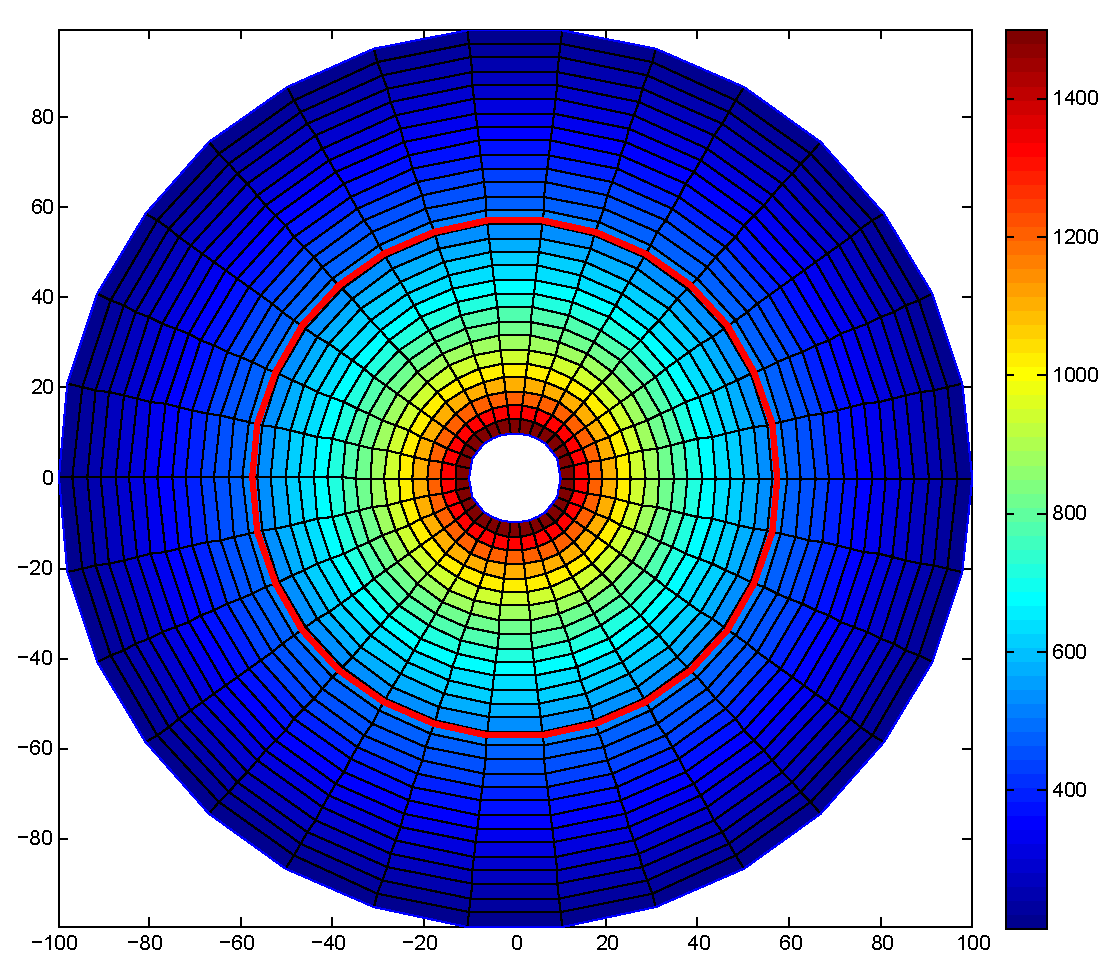
\includegraphics[width=1\textwidth]{figures/exp2-2.pdf}

\endminipage\hfill
\minipage{0.5\textwidth}

  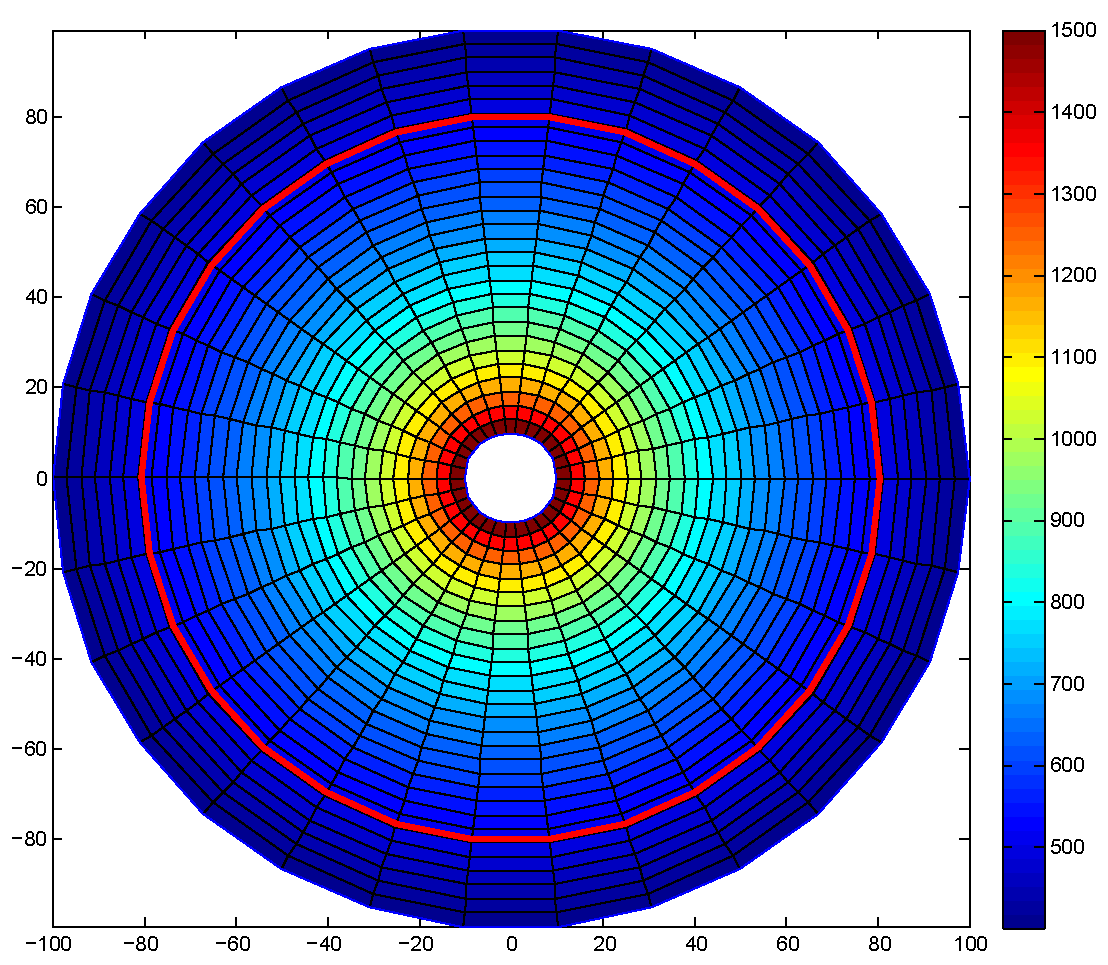
\includegraphics[width=1\textwidth]{figures/exp2-3.pdf}

\endminipage\hfill
\minipage{0.5\textwidth}

  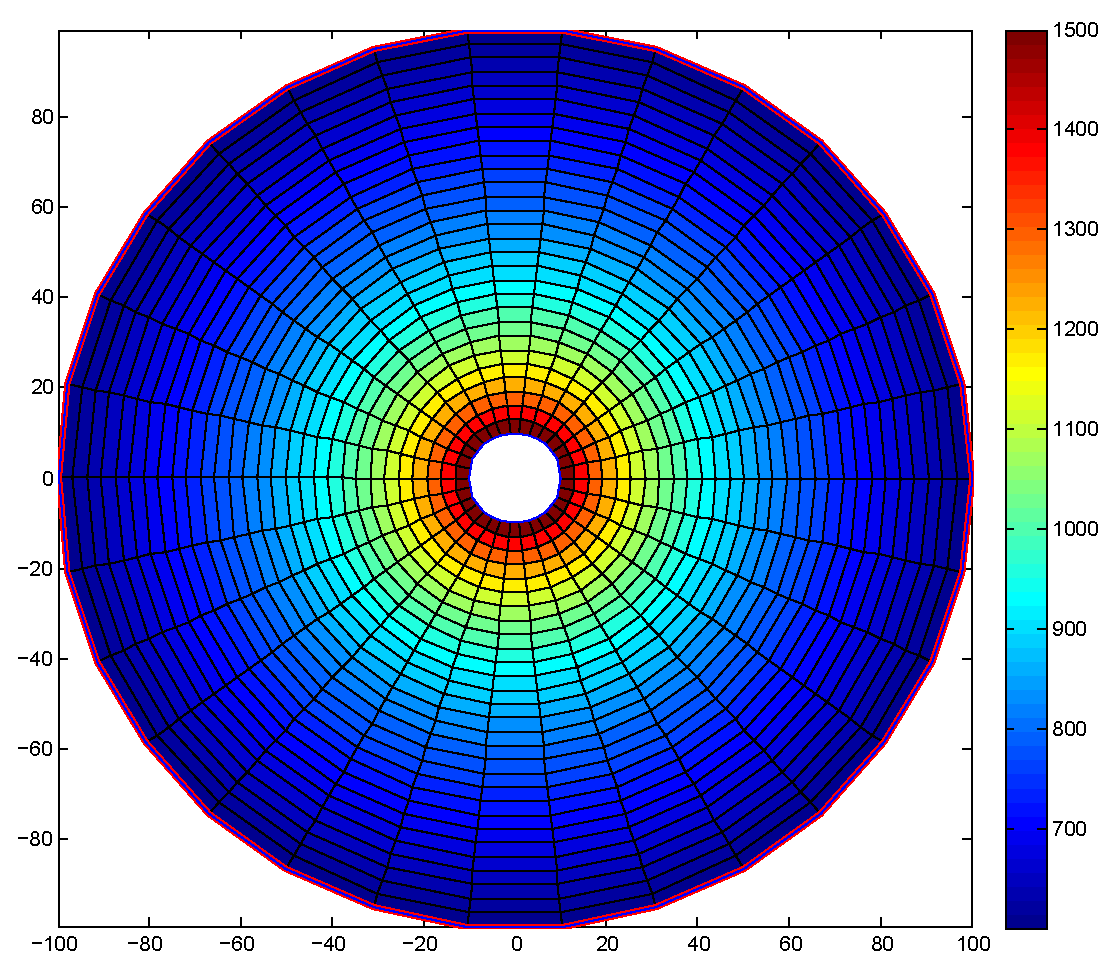
\includegraphics[width=1\textwidth]{figures/exp2-4.pdf}

\endminipage\hfill
\end{figure}

\clearpage

\begin{SCfigure}[1][ht!]
\sidecaptionvpos{figure}{t}
  \caption{ Se puede observar la comparaci\'on de performance entre eliminaci\'on Gausseana (GE) y factorizaci\'on LU con 20 instancias seguidas del mismo sistema. Como se visualiza, en la primera resoluci\'on del sistema el insumo de ciclos es casi el mismo, mientras que en las consecuentes la factorizaci\'on LU toma mucha ventaja con respecto a la eliminaci\'on Gausseana. Los resultados muestran un crecimiento lineal en funci\'on de la cantidad de instancias, ya que al haber fijado  el $n$ y el $m$ el insumo de ciclos en la resoluci\'on de una instancia es constante.\newline}
  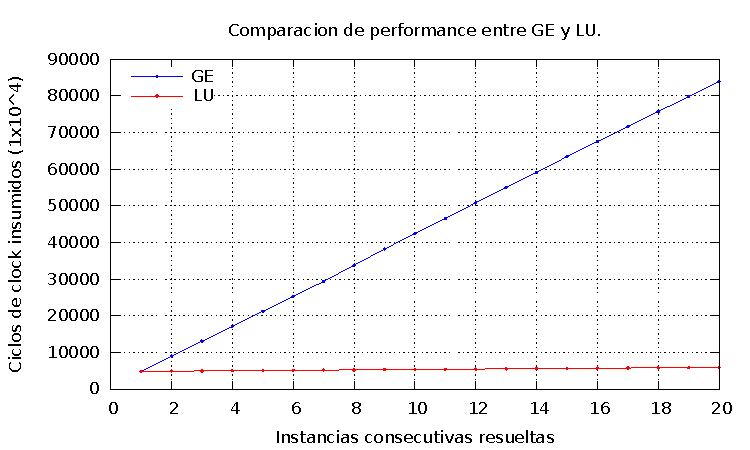
\includegraphics[width=0.6\textwidth]{../src/experimentacion/PDFs/compbench.pdf}
  \label{compbench-glu}
\end{SCfigure}

\begin{SCfigure}[1][ht!]
\sidecaptionvpos{figure}{t}
\caption{ En esta última experimentaci\'on intentamos realizar una comparativa que muestre mas claramente la diferencia de complejidad entre eliminaci\'on Gausseana y factorizaci\'on LU. Para ello realizamos $20$ iteraciones en las cuales $n=10$ para todas y $m$ era incrementado de a dos unidades en cada iteraci\'on (con un valor inicial de $10$). A la par de los incrementos de $m$ era incrementado $ninst$ de forma tal de que en las primeras iteraciones se pudiese observar con el algoritmo de LU un comportamiento mas cercano a una complejidad de $\mathcal{O}(n^3)$, mientras que en las ultimas iteraciones donde $ninst > 100$ el factor $n^2$ tomar\'ia mas importancia que la primera pero \'unica resoluci\'on con complejidad $n^3$.}
    \label{compbench-extra}
  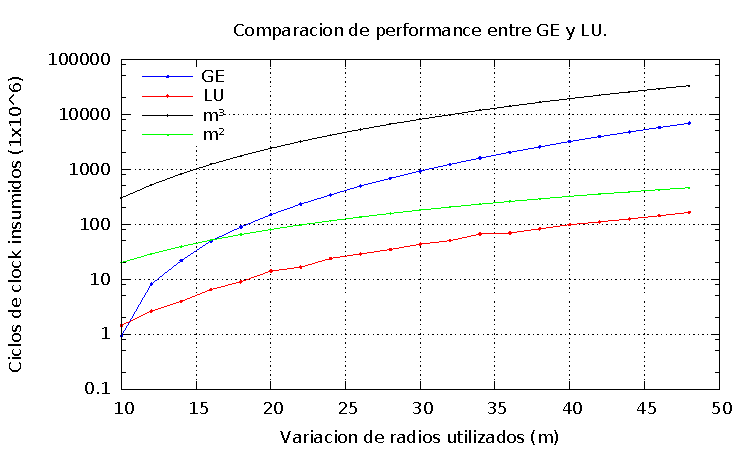
\includegraphics[width=0.6\textwidth]{../src/experimentacion/PDFs/compbench-extra.pdf}
\end{SCfigure}

